% Test

\documentclass[asi]{picINSA}

\usepackage{asi/vocabulaireASI}
%\usepackage{vocabulaire/vocabulairePicdyn}

\definecolor{gris}{gray}{0.75}% utilisé dans les annexes A B et C
\definecolor{gris2}{gray}{0.85}% utilisé dans les annexes A B et C

\titreAcronyme{Rapport de Stage Ingénieur}
\titreGeneral{Stage effectué chez Dynamease}
\titreDetaille{Performance et sécurité des applications Téléphoniques}
\sousTitreGeneral{Moreau Kévin\\Janvier - Juillet 2015}
\auteurs{Moreau Kévin}
\destinataires{Malandain Nicolas, Gasso Gilles, Nicolas Yves}
\resume{Le présent document résume le stage effectué au sein de l'entreprise Dynamease par Moreau Kévin}
\motsCles{Stage Ingénieur, ASI, Dynamease, Amélioration, Performance, Sécurité, Ios, Android, Aerogear, Docker}

%\SetWatermarkText{Brouillon}

\begin{document}
 \couverture{}
 \informationsGenerales{}


 \begin{center}
        \Huge{\bf Remerciements}\\[1.5cm]
\end{center}

Je souhaite exprimer toute ma reconnaissance à Yves \bsc{Nicolas}, créateur de Dynamease, pour m’avoir accueilli dans son entreprise, pour le temps qu’il m’a accordé, de son accompagnement tout au long de ce stage et également pour m'avoir donné son retour d'expérience en tant que chef de projet, créateur d'entreprises et développeur.

Par ailleurs, je remercie également mon collègue Etienne \bsc{Laplane} avec qui j’ai travaillé et mené à bien le développement de certaines fonctionnalités, des applications téléphoniques, réalisées durant ce stage.\\

Je remercie également Grégoire \bsc{Ternon}, consultant de Dynamease, pour m'avoir fait découvrir de nouvelles technologies et également pour son retour d'expérience en tant que jeune entrepreneur. 
 \tableofcontents

 \listoffigures
 \addcontentsline{toc}{chapter}{Table des figures}

 \chapter{Introduction}
 	Dans le cadre de ma formation ingénieur en Architecture des Systèmes d'Information, j’ai effectué un stage de fin d'année au sein de l'entreprise Dynamease située à Vernon (27200), du 26 janvier au 24 juillet 2015.

Au cours de ce stage j’ai pu m’intéresser à la création de nouvelles fonctionnalités, et au maintien des applications, sur deux systèmes d'exploitation téléphoniques différents, IPhone et Android. J'ai été responsable de la conception des applications jusqu'à leur mise à disposition pour les utilisateurs, en passant par l’intégration du design et aux mises à jour des services utilisés par les applications téléphoniques.

Ce stage m’a offert l’opportunité de découvrir les débuts d’une jeune entreprise en informatique porteuse d’un projet original et innovant pour le monde de la téléphonie et la communication professionnelle.

Par ailleurs, cette expérience m’a permis d’enrichir mes connaissances en informatique et plus particulièrement dans le monde du développement mobile, ainsi qu'au développement parallèle de fonctionnalités sur deux langages de programmation différents.\\


J’ai pu bénéficier de la double compétence de mon maître de stage, à la fois commercial et chef de projet informatique. J’ai pu, grâce à lui, comprendre au mieux les enjeux d’une startup informatique.

Lors de ce stage, j’ai eu l’occasion de travailler en équipe avec Étienne \bsc{Laplane}, un développeur en charge des serveurs de communication ainsi que d'une partie du serveur web Dynamease.
 	
 \chapter{Présentation de l'entreprise}
	\section{Présentation de Dynamease}

\subsection{Présentation du service Dynamease}

\subsection{Les différentes offres}

Dynamease propose à ses clients plusieurs offres. Chaque offre contient des fonctionnalité particulière. Ces offres suivent une hiérarchie, chaque offre contient les fonctionnalités des offres précédentes. La hiérarchie des offres Dynamease est la suivante :

[Diagramme hiérarchie]

Nous allons maintenant décrire les différentes offres.

\subsubsection{Basic}

L'offre Basic est une offre gratuite, elle permet à l'utilisateur d'accéder au fonction basique de l'application téléphonique et de l'application web, envoie de carte de visite Dynamease, liste de contact et pouvoir gérer manuellement sa disponibilité.

\subsubsection{Avantage}

L'offre Avantage s'adresse à des clients particulier, désirant avoir une gestion de sa disponibilité gérer par rapport à des calendrier (Calendrier Dynamease ou Google).

\subsubsection{Privilège}

L'offre Privilège permet aux utilisateur d'obtenir un numéro Dynamease. Ce numéro permet à l'utilisateur d'être joint sur n'importe lequel de ses appareils téléphoniques. Les appels dirigés vers le numéro Dynamease sont géré par le serveur Dynamease, celui-ci identifiera l'appel, défini sont importance et enfin le redirige vers l'appareil défini par l'utilisateur.

\subsubsection{Intégrale}

L'offre Intégrale est destiné pour les entreprises. Cette offre permet l'ajout d'employé qui détiendront un compte Avantage. Il est également possible d'ajouter des connecteurs. Les connecteurs permettent une meilleur identification d'appel ainsi qu'une meilleur redirection. Les connecteurs sont des données rentré par les entreprises qui donne des indications sur leurs clients ainsi que sur les employés responsable de ces clients.

\subsection{Présentation de l'environnement Dynamease}

 \chapter{Présentation de mon stage}
	Mon stage se déroulera pour l'essentiel sur la partie des applications téléphoniques de Dynamease. Il me sera également demandé de travailler sur les différentes méthodes de communication de Dynamease. Celles faisant intervenir, le serveur Dynamease avec les applications téléphoniques.

On peut séparer mon travail chez Dynamease en trois partie 

\section{Performance et amélioration}

J'aurais pour charge la mesure des performances, ainsi que les améliorations qu'il serait bon d'appliquer suite aux résultats obtenus par cette mesure. 

En ce qui concerne la recherche d'outils, je devrais tout d'abord réaliser une liste des différentes mesures que je devrais disposer pour avoir un aperçu des performances de Dynamease. De plus d'autre outils pourrait être ajouté à cette liste, des outils de vérification des installation informatique de Dynamease par exemple.

Une fois cette liste effectuée je devrais rechercher des outils réalisant les différentes tâches de cette liste, et les mettre en relation a fin de déterminer quels sont les meilleurs outils selon certains critère.

Une fois la liste des outils à utilisés créé, il faudra alors gérer leurs mise en place. Leur installation et leur configuration devront être effectué. Il me sera également demandé d'être capable de former quelqu'un à l'utilisation de ces différents outils.

Une fois la mise en place de ces outils effectuer j'aurais pour charge d'améliorer les fonctions ayant une mauvais performance. De plus certains dysfonctionnements sont déjà présent, je devrais également résoudre ces différents problèmes.

Pour le fonctionnement des différents outils de mesure je devrais également mettre en place un démarrage automatique de l'environnement de Dynamease.

\section{Ajout de nouvelles fonctionnalités}

Certaines fonctionnalités sont manquante dans les applications Dynamease. Il me sera demander de créer ces différentes fonctionnalités. Comme il l'a était dit précédemment, mon travail dans l'ajout de ces fonctionnalités se focalisera sur les application Dynamease ainsi que sur les procédé de communication entre le serveur et les applications. Il sera également possible que je modifie les différentes base de données pour répondre aux besoins des fonctionnalités.

Les différentes fonctionnalités a ajouter sont les suivantes :

\begin{enumerate}
	\item La réécriture de numéro;
	\item L'appel depuis l'historique d'appel;
	\item Le transfert d'appel;
	\item Le click2call.
\end{enumerate}

Chacune de ces fonctionnalités sera expliquer dans la partie des améliorations.

\section{Sécurité}
 
 \chapter{Apprentissage des technologies utilisées dans la réalisation des applications téléphonique}
 	\section{Introduction}

La réalisation des applications téléphoniques nécessitent différentes technologies et outils utilisés dans la création de ses applications. Les applications Iphone et Android nécessitant des outils différents, une partie non négligeable de mon travail a été de me former sur ceux-ci. A la suite de plusieurs recherches sur les documentations officielles j'ai pu noter les points suivant pour chacun des systèmes d'exploitation téléphonique.

Malgrès la différence de ces deux système d'exploitation, il existe quelques ressemblance, en particulier sur leur utilisation du pattern MVC (Model View Controler).Le modèle s’occupe de stocker les données, la vue les affiche à l’utilisateur, en créant les différents éléments de navigation et d'interaction. Enfin le contrôleur réalise le lien entre la vue et le modèle. Il récupère les informations de la vue, pour les stocker dans le modèle. Le modèle notifie le contrôleur pour que celui-ci mette à jour la vue.

\section{Technolgie utilisée pour Android}

\subsection{Les outils utilisés}

Pour réaliser des applications Android nous devons utiliser différents outils, que ce soit pour le développement ou pour la mise en production.

\subsubsection{Eclipse}

Eclipse est un IDE (Integrated Development Environment) permettant principalement le développement Java. Android étant réalisé en Java il est possible d'intégrer des plugin permettant le développement d'application Android avec cet IDE.

\subsubsection{Le playstore}
%eclipse
%android sdk
%playstore

\subsection{Le langage de programmation}

\subsubsection{Activity}

Une activité, au sens Android, est une classe permettant l’interaction avec l'utilisateur. Cette classe à la gestion de la création d'une vue ainsi que la gestion des actions que l'utilisateur établira sur cette vue. L'activité passe par plusieurs processus qui sont représentés sur le schéma suivant.

[mettre schéma Android activity]

On peut résumer tout ces processus en quatre états :
\begin{itemize}
	\item L'activité est au premier plan et peut être contrôlée par l'utilisateur (onResume -> onPause);
	\item L'activité est visible mais les controles de l'utilisateur ne sont plus pris en charge (onPause). Dans cet état toutes les données de l'activité sont conservées, mais en cas de manque de mémoire de la part de l'appareil téléphonique, l'activité est détruite;
	\item L'activité n'est plus visible elle est stoppée. Elle réagis de la même manière que dans un état de pause en ce qui concerne la mémoire des informations;
	\item L'activité est tuée, toutes ses informations sont effacées de la mémoire.
\end{itemize}
%%http://developer.android.com/reference/android/app/Activity.html#ActivityLifecycle

\subsubsection{Intent}

L'objet Intent permet le démarrage d'une activité ou d'un service. Un service réagis comme une activité qui n'aurai pas besoin d'interface utilisateur et qui tournerais en arrière plan. Ce démarrage peut être initié par n'importe quel composant de l'application.

\subsubsection{Manifest}
Le fichier Manifest représente les informations essentielle de l'application Android afin de créer le fichier APK nécessaire au lancement de l'application Android. Un fichier APK (Android PacKage) est un paquetage de fichiers compressés pour le système d'exploitation Android.

\section{Technologie utilisée pour IOS}

\subsection{Les outils utilisés}

\subsubsection{Xcode}
Xcode est l’environnement de développement intégré (EDI) permettant de développer les applications Apple (applications bureautiques et applications mobiles). Xcode est donc l’EDI de choix par défaut pour développer une application iOS. Xcode intègre un simulateur permettant d’émuler les périphériques (iPhone, iPad) de notre choix et d’exécuter l’application sans devoir passer par un périphérique physique bien que cela soit également possible. Pour ma part j'avais à disposition deux Iphones avec différentes version d'Ios afin de tester la compatibilité sur les IOS version 7 et 8. 

\subsubsection{Itunes Connect}
iTunes Connect est un site internet permettant de gérer les applications réalisée auprès d’Apple. Pour une entreprise, une fois enregistrée au programme de développement Apple, ce site permet de définir les membres de l’équipe de développent et leurs rôles au sein de l’équipe. Je possédais les permissions techniques qui permettaient de développer des application et de les publier sur l’Appstore. L'Appstore est la plateforme de téléchargement d'applications en ligne d'apple. ITunes Connect permet aussi de définir l’ensemble des métadonnées qui seront présentées aux utilisateurs lors de leur achat de l’application sur l’AppStore (mots-clés, descriptif, captures d’écrans, prix ..).

Ce site permet également d'avoir un retour sur les utilisateurs de l'application (commentaire, nombre de téléchargement, note obtenue sur l'application ...)


\subsection{Le langage de programmation}

\subsubsection{Delegate}

L'objet délégant garde une référence sur l'objet (le délégué) à qui, il va déléguer certaines actions. La délégation se fait par l'envoi d'un message. Le message informe le délégué. Le message est ensuite traité par le délégué. Le délégué pourra répondre à ce message en renvoyant un résultat ou en mettant à jour une vue. Le système de délégation a été utilisé afin de faire transiter des informations entre les différentes vues de l'application développée. La délégation s'effectue par la définition d'un protocole décrivant les messages envoyés entre les objets.

Pour utilisé une délégation, un objet doit hériter d'un autre objet \textit{delegate}. Cette héritage pourra nécessiter une redéfinition des méthodes voulues par le développeur. Si certaines méthodes ne sont pas redéfinies, alors une méthode par défaut définie dans l'objet \textit{delegate} sera appelé. On peut comparer se procédé à une interface Java à la différence que toutes les méthodes n'ont pas à être définies.

\subsubsection{Block}

Un \textit{block} permet de définir une fonction, qui pourra être utilisée en tant que paramètre dans une autre fonction ou méthode. Ceci peut être utile lors de l'appel de méthode asynchrone qui nécessite le traitement de données reçues ou le démarrage d'un autre processus.

 \chapter{Performance}
	\section{Gestion des Notifications Téléphoniques : Aerogear}

Les notifications sont très importante pour l'application téléphonique Dynamease. En effet ce sont grâce à celles-ci que les informations sur l'appelant sont récupéré par l'appareil. 

\subsection{Fonctionnement des notifications Push}

Une notification est un message envoyé à un smartphone. Ce message à la possibilité de réveiller le smartphone et d'afficher une information. L'envoie d'une notification passe par une plateforme. Pour envoyer une notification à un appareil Android il faut passer par Google Cloud Messaging (GCM). Pour les appareils IOS il faut passer par Apple Push Notification Service (APNS).

Pour cet ensemble de plateforme le fonctionnement est quasiment identique. L'appareil doit s'inscrire à la plateforme correspondante.
Durant cette inscription l'appareil obtient un identifiant unique. Les messages qui lui sont envoyés sont de la forme d'un objet Json (bien que pour Android il soit également possible de passer par un objet de type texte). Les notifications sont utilisés pour envoyer une information à afficher à l'utilisateur (encore une fois pour Android il est également possible d'envoyé une notification pour demander à l'application de se synchroniser sans pour autant afficher de message).

\subsection{Principe d'Aerogear}

Aerogear est une application serveur qui permet l'envoie de notification Push vers différents systèmes d'exploitation téléphonique. En ce qui nous concerne il s'agit d'un envoi vers les systèmes Android et IOS.

L'utilisation de l'API de ce serveur, permet d'envoyer des requêtes vers le serveur Aerogear. Celui-ci aura pour charge de transformer cette requête en une requête adapté pour le système d'exploitation vers lequel la requête doit être envoyée.

Ce procédé permet de délégué l'envoie des notifications Push. Une requête unique permet l'envoie de notification plutôt que d'avoir à effectuer une requête pour chacun des systèmes d'exploitation. De plus le serveur se charge également du stockage des informations des différents systèmes d'exploitation de chaque client.

Les requêtes Aerogear permettent également l'envoie de notification vers toutes les installations, ainsi que l'envoie vers toutes les installation d'un variant spécifique.

\subsubsection{Définitions} 

Avant de décrire le fonctionnement du serveur Aerogear il nous faut définir les différents terme suivant :

\begin{description}
 \item[Application Push :] Représente une application téléphonique ayant recours à des notifications Push.
 \item[Variant :] Représente une plateforme téléphonique comme IOS ou Android. Une application Push peut avoir plusieurs variants. Plusieurs variants peuvent représenter une seule plateforme. Le variant permet de stocker toutes les propriétés nécessaire à l'envoie de notification Push, comme le $"\textit{Google API key}"$ pour Android.
 \item[Installation :] Correspond à une application téléphonique s'étant inscrite sur un variant. Chaque variant peut avoir plusieurs installation. Une installation contient toutes les informations nécessaire à l'envoie de notifications, comme l'id du téléphone.
 \item[Alias :] Correspond à l'identifiant d'une installation.
\end{description}

\subsubsection{Fonctionnement}

\begin{figure}[!h]
	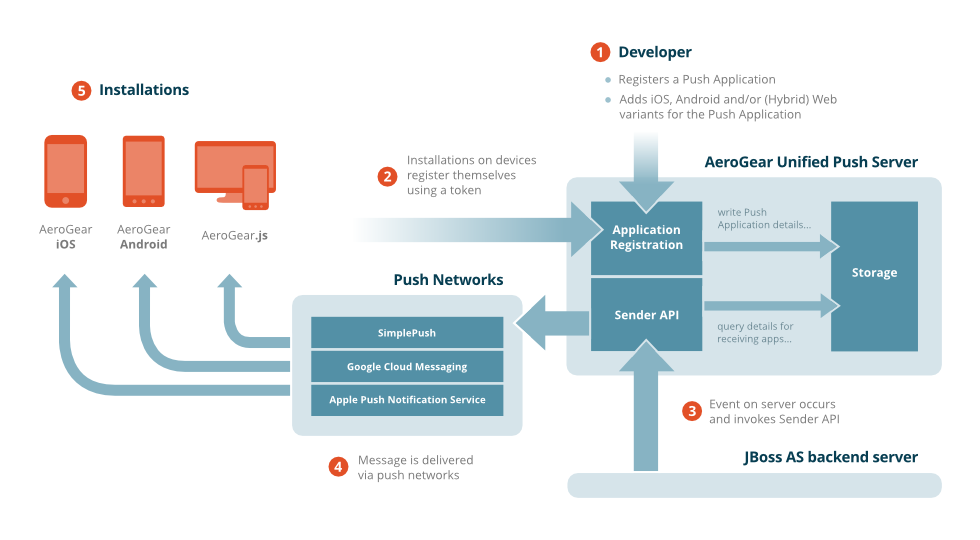
\includegraphics[scale=0.6]{img/aerogear_unified_push_server.png}
	\caption{\label{aerogear} Fonctionnement d'Aerogear}
\end{figure}

Le fonctionnement du serveur Aerogear suit le schéma précédent.

\begin{enumerate}
 \item L'administrateur doit commencer par créé une application Push, qui doit contenir au moins un Variant;
 \item L'application téléphonique demande un enregistrement en envoyant toutes les informations nécessaire à Aerogear. Ces informations sont stockées.
 \item Une requête est envoyé à  Aerogear dans le but d'envoyer une notification vers l'installation correspondant a un alias. Aerogear récupére toutes les informations nécessaire. La requête Push est ensuite traduite vers la plateforme correspondant au système d'exploitation correspondant à l'alias. La requête est ensuite envoyée vers la plateforme appropriée.
 \item C'est maintenant la plateforme qui se charge de l'envoie de la notification vers l'installation correspondant à l'alias.
 \item L'installation reçois la notification, et c'est à l'application téléphonique de gérer le traitement de cette notification.
\end{enumerate}

Les requêtes Aerogear permettent également l'envoie de notification vers toutes les installations, ainsi que l'envoie vers toutes les installation d'un variant spécifique.

\subsection{Mise à jour d'Aerogear}

Mon premier objectif au niveau d'Aerogear était de mettre à jour cette plateforme. Pour ce faire je me suis rendu sur le site officiel afin de connaître les différentes procédure de son installation.

Le serveur Aerogear se présente sous la forme d'un fichier war. Il faut savoir que pour fonctionne, Aerogear à besoin d'un serveur Jboss et d'un base de données. Aerogear peut fonctionner avec différentes base de données SQL (H2, Mysql et postgreSQL). La base utilisée par Dynamease étant une base de données MySQL j'ai donc choisi d'installer la version correspondante.

Plusieurs problème se sont accumulé durant cette installation, en effet des erreurs se produisaient durant le lancement du serveur. Après plusieurs recherche il s'est avéré que le lien donné durant le processus d'installation pointé vers les sources d'une version non stable du projet. Après avoir récupéré un projet stable, j'ai du faire face à une autre difficulté. Le serveur n'arrivait pas à utiliser la base de données MySQL. Après avoir effectué d'autre recherche il a semblait que la version utilisée éprouvé quelques difficultés avec les bases de données MySQL et PostgreSQL, et que seul les base de données de type H2 pouvait être gérées.

Les base de données H2 fonctionnent sous un environnement Java. Afin de pouvoir y accéder de façon graphique le logiciel officiel de cette base de données sera installer également sur le serveur pour pouvoir accédé plus facilement aux données s'y trouvant. Ainsi l'administrateur système pourra aisément réaliser ses requêtes de la même manière qu'il les aurait effectué sur une base de données MySQL.

Après son installation j'ai eu pour objectif de réalisé une Image Docker d'Aerogear. L'explication de cette réalisation sera faîte lors de la partie sur Docker.

\subsection{Mise à jour des notifications}

Après la mise à jour du serveur Aerogear j'ai également dû réaliser des mises à jour du côté des applications téléphonique.

Pour les applications IOS, une mise à jour était nécessaire du fait que certaines méthodes utiles pour l'enregistrement vers le serveur des notifications n'étaient pas rétrocompatible entre la version 7 et la version 8. Comme nous devions garder une version de l'application pour les personnes ayant encore une version IOS7 une vérification de la version de l'appareil est effectué avant tout enregistrement au serveur. Mais il est très probable que l'application Dynamease devienne, dans le futur, inaccessible pour les personnes possédant une version 7 d'IOS. En effet la version 8 permet beaucoup plus de liberté au niveau des notification notamment la possibilité d'ajouter des bouton d'action aux notifications.\\

L'autre mise à jour effectuée est la forme d'envoie des notifications. L'ancienne version envoyé les informations sous la forme de chaîne de caractère. Ces chaînes de caractère était difficile à traité du fait que les informations pouvait être dispersées. La solution la plus évident à mettre en place était de faire passer des objets Json au travers les notifications. En effet, les objets Json sont très facile à créé, à déchiffrer et de plus peuvent être écris sous la forme d'une chaîne de caractère spéciale.

Grâce à cette méthode il est plus facile d'effectuer un traitement sur les informations reçus et de dédier à l'application téléphonique le tri des informations et l'affichage de celle-ci.

\section{L'environnement Docker}

\subsection{Fonctionnement de Docker}

Docker est un logiciel open source qui permet l'automatisation du déploiement d'application sur n'importe quel serveur Linux. Docker réuni une application et ses dépendance dans une container virtuel qui permet la portabilité de cette application facilement. En effet, la configuration nécessaire au fonctionnement d'un application sera déjà présente dans ce container. Ce container pourra être utilisé aussi bien sur une machine locale que sur un serveur, sans nécessité de configurer la machine qui fera tourner l'application. 

Docker propose également un serveur Hub dans le but de partager les différentes application Docker réalisé par les utilisateurs Docker.

Docker contrairement aux machines virtuelles n'a pas besoin de démarrer un système d'exploitation. Docker utilise directement le système d'exploitation de la machine sous-jacente. Docker exécute également ses processus de façon isolée.

Avant de continuer la présentation de docker, une définition de quelques termes doit être effectuée. 



\subsubsection{Container}

Le container est l’exécution d'une application se trouvant sur docker. Chaque container, détiens une adresse IP privée.


\subsubsection{Images}

Une image Docker est la configuration d'une application au sein de Docker. Cette image peut être stocké sur le Hub de Docker afin que celle-ci soit partagée avec d'autre utilisateur. Pour réaliser une image Docker, il faut rédiger un Dockerfile. Le Dockerfile représente le plan de fabrication de l'image docker. Ce fichier doit contenir toute les dépendances nécessaire au fonctionnement de l'application. Ce fichier peut être représenté comme un script qui sera exécuter dans la création de l'image. Il faut réaliser ce script en prenant bien en compte qu'il s'agit de la configuration de l'environnement et non pas du lancement de l'application. Il est tout de fois possible de définir un script qui sera réalisé lors de l'exécution du container.

Le Dockerfile doit aussi configurer les ports qui doivent être ouvert sur le container. Par exemple pour un serveur Tomcat accessible depuis le port 8080, il faudra indiquer au Docker que la port 8080 du container doit être accessible. A l'exécution du container, il est possible d'indiquer le port de la machine local qui sera redirigé vers un des ports du container. 

Cette image Docker nécessite d'abord de partir d'une image Docker de base. Par exemple pour réaliser l'image d'un serveur Jboss, nous avons besoin de Java, nous partirons donc d'une image Docker Java.


\subsubsection{Volume}

Un volume est un lien entre un répertoire se trouvant dans le container et un répertoire se trouvant sur la machine faisant tourner le container. Ainsi on peut utiliser des fichiers se trouvant dans un dossier en local, dans le container. Le volume peut également être utilisé pour récupérer des fichiers se trouvant dans le container. Il est également possible de lier les volumes d'un container dans un autre container.

Les volumes sont à définir dans le Dockerfile en indiquant le répertorie du container qui contient les volumes.

\subsubsection{link}

Le \textit{link} est un lien entre deux container. Comme nous l'avons vu précédemment, il est possible d'accéder à un port du container depuis un port de la machine locale. Il est également possible d'indiquer un lien entre deux docker pour que ceux-ci communique comme s'ils étaient sur deux serveurs différents. Le \textit{link} va donc ré-écrire dans le fichier host du container qui définiera le nom du container à lier avec son adresse IP.

\subsection{Réalisation Docker pour le compte de Dynamease}

\subsubsection{Aerogear}

Comme nous l'avons vu précédemment, Aerogear nécessite d'un serveur JBOSS pour son fonctionnement. Nous allons donc partir d'une image JBOSS pour la réalisation de l'image Aerogear. L'accès à se serveur se fera obligatoirement par le port 8080, car une vérification au niveau de KeyCloak est réaliser entre le port par lequel le port entre et le port par lequel l'application écoute.

Un volume sur les fichiers de base de données H2 sera également mis en place afin de pouvoir accéder à cette base de données, pour toute importations, exportation ou modification de données. 

\subsubsection{Nginx}

Nginx est un reverse proxy, qui permet de rediriger les requêtes entrante sur un serveur vers un autre serveur distant, où vers un autre port du même serveur.

Pour fonctionner Nginx ne nécessite que d'une distribution Linux. Debian est donc préféré aux autres distribution car c'est celle-ci qui est préféré pour tout serveur.

Le port d'accès par défaut à Nginx est 80. Ce port sera donc ouvert par le container, mais il est libre à l'utilisateur de ce container de redéfinir, lors du lancement du container, le port par lequel on accédera à ce container.

Un volume sera également créé vers le répertoire où sont stockés les fichiers de configuration Nginx, afin que la configuration Nginx, ne dépende pas d'une image mais d'un container.

\section{Démarrage automatique d'un environnement de travail}

\subsection{Fonctionnalités attendues}

Ce procédé doit permettre aux développeurs de Dynamease de pouvoir mettre en place de façon rapide et automatisé, un environnement de travail complet permettant l'accès aux différents services de Dynamease. 

Il doit également être possible de pré-remplir les bases de données Dynamease, avec des données provenant de base de tests déjà utilisé ou bien d'une base de production.

L'outil ainsi créé devra pouvoir être utilisé aussi bien sur des serveurs que sur les machines locales des développeurs. 

\subsection{Étude du cahier des charges}

Les environnements utilisés par Dynamease peuvent tourner grâce à des container Docker. Pour l'outil qui sera développer, l'utilisation de ces containers sera mise en avant. Il sera donc nécessaire de déterminer l'ordre d'exécution de ces containers, en déterminant les différentes dépendance de ces containers.\\

Il faut également déterminer quels sont les meilleurs solutions pour la mise en place d'un système permettant l'intégration de données au démarrage de l'environnement Dynamease. L'environnement complet de Dynamease est constitué de plusieurs sous environnement, les différents environnement qui nécessitent d'un intégration de données sont :

\begin{itemize}
	\item La base de données MySQL;
	\item La base de données Ldap;
	\item La base de données liée à Aerogear;
	\item Les fichiers de configuration du serveur Dynamease.
\end{itemize}

Il faudra donc déterminer, pour chacun de ces environnement, quels sont les techniques permettant une intégration de données.

De plus il doit être possible de démarrer d'un environnement vide, il faudra donc gérer ce cas de figure, en initialisant les bases de données de manière à ce qu'elles soient utilisable dans l'environnement complet de Dynamease.

\subsection{Réalisation de l'outil}

\subsubsection{Détermination des dépendances}

[Mettre Diagramme pyramide]

Nous allons étudier le diagramme ci-dessus, de manière descendante. Tout en haut nous avons l'environnement Nginx, celui-ci nécessite la mise en place des environnements Tomcat et Aerogear pour fonctionner. L'environnement Tomcat nécessite l'existence des bases de données MySQL et Ldap. 

Donc il nous faudra lancer l'environnement l'ordre suivant :

\begin{enumerate}
	\item La base de données MySQL;
	\item La base de données Ldap;
	\item Aerogear;
	\item Tomcat;
	\item Nginx.
\end{enumerate}

\subsubsection{Récupération et utilisation des données}

Le fonctionnement de l'environnement Dynamease dépend de plusieurs données, on doit donc récupérer ces données. On peut séparer les données à récupérer en deux catégories, les données de configuration et les données de stockage d'informations.

Les données récupérées, par le serveur Tomcat de Dynamease, sont essentiellement des données de configuration. Cette configuration permet à Dynamease de connaître les adresses internet des différents services nécessaire à son fonctionnement. Ces adresses peuvent être différentes d'un environnement à un autre selon l'emplacement de démarrage de l'application Dynamease. Le mieux est donc d'avoir ces fichiers stockés sur l'emplacement de démarrage.

Pour ce type de données, il sera demandé la création d'une variable d'environnement par l'utilisateur afin de lui permettre de préciser à l'outil, l'emplacement des différents fichiers de configuration de Dynamease. 

Des fichiers de configurations par défaut seront présent dans l'outil. Si l'utilisateur ne désigne pas de répertoire contenant ces fichiers de configurations, un message sera affiché pour le prévenir que les fichiers de configuration par défaut seront utilisés, mais que cela peut entraîner quelques dysfonctionnement.\\

En ce qui concerne les données des différentes bases de données, celles-ci peuvent être stockées indépendamment de leur bases de données d'origine. Seul leur intégration sera différente.

Il nous reste donc trois base de données à remplir avec nos fichiers de données. Leur technique d'intégration étant différente nous allons les étudier pour chaque base de données. 

[Explication schéma ?] 

Deux solutions de stockage peuvent être étudiés, on pourrait utiliser les volumes de chaque containers, en intégrant les données. Cette méthode risque d'être assez limité sachant que chaque utilisateur devra disposer des fichiers de données afin de les intégrer dans son environnement. La seconde solution serait d'utiliser une nouvelle image Docker qui aura pour rôle le stockage de tout les fichiers de données. Cette solution permettrait de pouvoir utiliser n'importe quelle base de donné sans récupérer les fichiers de données. C'est cette seconde solution que nous allons développer par la suite.

Cette solution prend en compte que le container de données contienne des volumes pour stocker les fichiers de données. Or, comme nous l'avons vu précédemment, les volumes créés des liens symboliques depuis les volumes du container vers les répertoires situés sur la machine faisant tourner le container. Donc le container serait opérationnel uniquement sur la machine l'ayant créé, si ce container se trouve sur un autre système, il se peut que les liens ne pointes sur aucuns fichiers ou sur de mauvais fichiers. 

On a également vu qu'on pouvait exécuter des commandes lors de la création du container. L'idée est d'utiliser un script de démarrage du container, qui nous servira à déplacer et trier les fichiers de données vers de nouveaux répertoires.

Grâce à cette récupération nous pouvons maintenant faire un traitement pour chaque fichier selon le type de base de données où celui-ci doit être inclue.\\

Il est aussi prévu de permettre aux utilisateurs de cet outil de lancer un environnement de travail, vide. C'est à dire seulement avec les bases de données initialisées, mais sans données. Pour cela l'image du docker de stockage des données sera généré avec les fichiers d'initialisation de chacune des bases de données. Un script de démarrage aura pour rôle de déterminer si des fichiers d'intégration de données sont présente, si c'est le cas, ces fichiers seront déplacé vers le répertoire correspondant à la base de données, sinon se seront les fichiers d'initialisation qui y seront placés. 

\subsubsection{Récupération de la version Dynamease}

Le lancement de l'environnement de travail Dynamease, doit être précisé d'un numéro de version du serveur Dynamease. 

Chaque version de Dynamease est présent sur le \textit{repository} Docker de Dynamease. Chaque nouvelle version déposé sur le serveur Git est récupérée par le serveur Jenkins. Celui-ci aura pour charge de vérifier le bon fonctionnement de la version déposée. Si celle-ci est correcte alors une nouvelle image Docker du serveur est créée avec le nom du commit comme numéro de version.

La création d'une image docker Dynamease, nécessite d'abord la compilation de l'ensemble du code source de Dynamease, de la récupération des archives (war) du serveur et enfin de leur intégration vers la nouvelle image Docker.

Le script de démarrage de l'environnement prendra en paramètre un numéro de version. Il vérifiera alors si l'image est présente en local, si ce n'est pas le cas l'image sera télécharger depuis le serveur Docker.

Grâce à cette méthode, il est possible de démarrer rapidement n'importe quel version de Dynamease.

\section{Amélioration des applications téléphoniques}

Nous allons maintenant aborder les différentes améliorations que nous devions réaliser après la réalisation de plusieurs tests de performance.

\subsection{Récupération des contacts Ios}

En début de stage un problème nous a été reporté par un utilisateur de l'application Iphone. L'application ne démarrer pas sur son Iphone. En effet tout de suite après la connexion de l'utilisateur, l'application se fermer subitement. Nous avons donc tenter de reproduire ce dysfonctionnement sur nos téléphone de test. Pourtant il nous était impossible de déterminer d'où venait l'erreur.

Nous avons donc demander le modèle d'Iphone et la version IOS de l'Iphone afin de pouvoir reproduire la procédure d'erreur dans les mêmes conditions. Mais encore une fois l'application semblait très bien fonctionner sur nos téléphone de test. Nous avons également demander à l'utilisateur de se connecter à l'aide d'un de nos téléphone de test, mais l'erreur ne s'est pas reproduite.

Nous en avons donc conclu que l'erreur devait provenir d'une configuration spéciale de l'Iphone de l'utilisateur.

Nous avons donc lister les différentes méthodes exécutée par l'application au démarrage, afin de déterminer celle qui aurait pu interagir directement avec une configuration spéciale de l'utilisateur.

[Diagramme de Mise en service de l'application]

Les différentes méthodes exécuter par l'application étaient, la récupération des informations de l'utilisateur auprès du serveur Dynamease, la récupération des contacts du portable et l'inscription sur le serveur Aerogear.

Après une observation sur les logs des serveurs Dynamease et Aerogear, nous nous sommes aperçus que les données de l'utilisateur été bien envoyé mais que le serveur Aerogear ne recevait pas de requête d'inscription.

L'erreur provenait donc de la récupération des contacts. De plus nous avons remarquer que l'utilisateur avait énormément de contact. Le problème pouvait donc provenir soit d'un contact particulier de l'utilisateur dont les informations étaient mal traitées, ou bien que le nombre important de contact faisait fermer subitement l'application.

Pour éviter de demander la liste de contacts de l'utilisateur nous avons décider en premier lieu de se pencher sur la seconde solution en créant des centaines de contact que nous importerions par la suite dans le téléphone de test. L'application arriva parfaitement à traiter ces centaines de contact.

Nous avons donc du demander la liste de contact de l'utilisateur dans le but de détecter quel était le contact qui produisait cette erreur, et quelle était la cause.

Après l'importation de ces contacts, nous avons remarqué que l'erreur se produisait également  sur les téléphones de tests. Après une observation des logs généré par l'application il est apparu qu'il existait un contact dont le nom commencé par le caractère $'@'$.

Les contacts dans l'application Iphone sont stocké dans un dictionnaire (ensemble clefs valeurs). Les clefs sont représenté par le noms de l'utilisateur et les valeurs sont les informations relative à l'utilisateur. La clef est donc de type chaîne de caractère. Or en Objective-C le caractère $'@'$ est un caractère spécial. L'Iphone n'arrivant pas à interpréter ce caractère l'application ferma subitement.

Afin de régler ce type de problème, un caractère spécial $'\textbackslash'$ est ajouté devant chaque caractère spécial pouvant être trouvé dans le nom ou les informations clients. Ce caractère à pour fonction, dans l'Objective-C de signifier à l'application de ne pas interpréter le caractère spécial qui le suit. 

\subsection{Recherche et récupération automatique des contacts}


\subsubsection{Recherche de contact}

L'application Téléphonique Android, permet aux utilisateurs d'avoir une liste de contact. Cette liste de contact est triée par défaut dans l'ordre alphabétique par rapport aux noms de famille des contacts. De plus une barre de recherche est disponible pour faire une recherche dans cette liste.

La version précédent ma correction, n'effectuait la recherche uniquement sur le nom, de plus sur de longue liste de contact, la recherche pouvait prendre beaucoup de temps.

La première étape pour effectuer une correction est d'observer la technique utilisait pour cette recherche, ainsi que les différents procédés utilisés par la liste de contact.\\\\



En premier lieu j'ai étudié les différents moyens de stockage que proposait Android. Celle-ci propose trois moyens de stockage qui sont :

\begin{enumerate}
	\item Stockage par le biais de clef valeur;
	\item Stockage dans un fichier texte;
	\item Stockage à l'aide d'une base de données SQL Light.
\end{enumerate}

La première technique peut être utilisée pour de petites valeurs uniques, comme le nom de l'utilisateur, son numéro de téléphone, etc.

Le fichier texte est surtout utilisé si on doit générer des fichiers de données, pouvant être récupéré par l'utilisateur.

La base de données SQL est utilisé pour stocker des liste de données suivant le même schéma.

C'est cette dernière option qui nous intéresse pour le stockage de la liste de contact. C'est effective cette technique de stockage qui est utilisée pour le stockage des contacts.

Un contact normal est représenté par son nom, son prénom, son numéro de téléphone. Un contact Dynamease est représenté par son nom, son prénom et son Id Dynamease. C'est deux type de contact son stocké dans la même table de données, et son différencié par une variable booléenne qui est à vrai si le contact est un contact Dynamease et est à faux sinon.\\\\

L'algorithme anciennement utilisé pour la recherche des contacts suivait le diagramme suivant :

[Mettre diagramme]

A chaque fois que l'utilisateur entre une lettre dans la barre de recherche, le processus de la recherche est lancé. Pour chaque contact de la liste, on vérifie si l'ensemble des lettres, entrées dans la barre de recherche, est présent dans le nom du contact. Si on trouve une correspondance entre l'ensemble des lettres et le nom du contact on ajoute ce contact à la liste de retour. Et on effectue cette correspondance pour chaque contact.

Ce processus est long en raison la recherche sur toute la liste de contact à chaque ajout de lettre dans la barre de recherche. L'autre problème flagrant est que la recherche n'est effectué que sur le nom.\\\\

La première résolution de ce problème suit le processus suivant :

[Mettre Diagramme]

Avant toute recherche la liste de contact est contenu dans le résultat à retourner. Par défaut tout les contacts correspondent à une recherche vide. A chaque ajout de lettre, on recherche dans la liste dernièrement retournée les contacts ayant l'ensemble des lettres de recherche dans leur prénom ou dans leur nom. Si une correspondance est trouvé alors le contact est ajouté dans une liste temporaire. Une fois tous les contacts vérifiés, on remplace la liste de résultat par la liste temporaire, et on renvoie la liste de résultat. Et on continue sur le même principe à chaque ajout de lettre\\\\

Le problème de cette solution c'est que l'ordre des mots de recherche est importante faire une recherche $"\textit{nom prénom}"$ ne sera pas interprété de la même façon que la recherche $"\textit{prénom nom}"$.

[Mettre diagramme]

On reprend le même principe que précédemment, mais cette fois-ci on fait un travail supplémentaire entre l'ajout d'une lettre et la recherche dans la liste de contact. On sépare les différents mots de la barre de recherche. Pour la estime qu'il y a un nouveau mot à chaque fois que la barre espace est pressée. Ensuite la recherche dans les contacts doit correspondre à chaque mot de la barre de recherche. Si un mot ne correspond pas, alors le contact ne sera pas ajouter à la liste de résultat. Tous les mots doivent correspondre, pour que le contact soit ajouter dan la liste de résultat.

\subsubsection{Récupération des contacts du téléphone}

La récupération des contacts ne semblait s'effectuer qu'une seule fois, lors du premier lancement de l'application. De plus il existait quelques problème au niveau du temps de récupération des contacts. Plus la liste de contact était grande et plus le temps de récupération était longue (par exemple pour une liste de contact de 10000 contacts le chargement pouvait être de quelques jours).\\

Après une inspection du code, l'activité de la liste de contact se chargé de la récupération des contacts à chaque lancement de cette activité. Or cette récupération avait une mauvaise condition pour la récupération des contacts.

La liste de contact est stockée par ordre alphabétique dans la base de données de Dynamease, c'est également le cas pour la liste de contact du téléphone. L'activité vérifie que le nombre de contacts dans la liste de contact du téléphone est égale au nombre de contact de la liste de contact de l'application Dynamease. Si ce n'est pas le cas une vérification est effectuée. Le problème se situe sur la suite du procédé. Le cursor permettant la récupération est programmer pour récupérer les contacts en partant de l'index correspondant au nombre de contact dans la liste de contact Dynamease moins un. Or les contacts stockés dans la base de données du téléphone ne sont pas trié par ordre chronologique mais par ordre alphabétique. Donc si un contact, ajouté à la suite du premier démarrage, est ajouté au début de la liste de contact, alors il ne sera jamais récupéré, et le programme fera une récupération de contact à chaque démarrage de l'activité.

La recherche est maintenant effectuée sur l'ensemble de la liste de contact du téléphone est une vérification sur l'existence des contacts est également effectuée, afin de ne pas avoir de doublon.\\ 

La récupération des contacts s'effectue par des \textit{Task}. Comme un \textit{Thread}, plusieurs \textit{Task} peuvent être en fonction "simultanément". Donc à chaque fois que l'activité de la liste de contact est lancée, la \textit{Task} de récupération des contacts est lancé. Donc le temps processeur est divisé entre ces deux \textit{Task}. Pour améliorer cette récupération une condition est rajouter pour déterminer si une récupération est déjà en cour afin de ne pas re-diviser le temps processeur. De plus un bouton d'actualisation de la liste de contact a été ajouter. Dorénavant, la récupération des contacts s'effectue seulement si la liste de contact de l'application Dynamease est vide ou si l'utilisateur appuie sur le bouton d'actualisation.

\subsubsection{Récupération des images de profile}

Il est apparu également qu'à chaque affichage de la liste de contact, dans l'application Android, une requête pour récupérer les images de profiles Dynamease est envoyé. Ces requêtes n'ont pas forcément lieu d'être effectuées à chaque affichage. En effet, le changement d'image de profile est beaucoup trop rare pour qu'une requête soit envoyé aussi couramment.

La requête de récupération des images s'effectue grâce à une requête Json. Le résultat de la requête se présente sous la forme d'une suite de caractère représentant l'image. Cette récupération est effectuée pour l'affichage des images dans la liste de contact. Il faut donc trouver une solution pour ne pas avoir à effectuer une requête pour l'affichage des images.

Le plus simple est de stocker les images sur l'appareil de l'utilisateur. Nous avons exploré précédemment les différentes techniques de stockages qu'offrait Android. La meilleure solution est d'utiliser l'écriture de fichier. Ce type de stockage, effectue, par défaut, la sauvegarde dans un dossier spécifique à l'application.On récupérera donc la suite de caractère pour la stocker dans un fichier. 

La récupération des images doit au moins être effectué une fois. Pour cela on suivra l'algorithme suivant :

[mettre Diagramme]

Lors de l'affichage de la liste de contact, à chaque contact Dynamease on fait la vérification suivante. On vérifie si l'image de profile est présente dans le répertoire de l'application Dynamease. Si l'image n'est pas présente, on envoie une requête vers le serveur Dynamease, afin de la récupérer. Une fois cette image récupérée, on stocke la suite de caractère récupérée dans un fichier. Le fichier de sorti aura sera nommé comme l'Id Dynamease du contact.

Ainsi l'affichage des images se fera par le biais de la récupération des fichiers images présent sur l'appareil téléphonique.

\subsubsection{Amélioration possible}

La récupération des images ne se fait qu'une seule fois. Or il est possible qu'un contact change son image de profile. Aucune mise à jour ne sera effectuée avec la méthode actuelle. Il faut donc penser à une solution pour que les images de profiles soient mises à jours. Pour cela on pourrait utiliser le bouton de rafraîchissement de contact déjà utilisé pour mettre la liste des contacts du téléphone à jour. 


\section{Amélioration continue du services par la mise en place d'outils}

La mise en place d'outils d'aide à la mesure des performances est importante pour les entreprises afin de leur permettre d'affirmer le bon fonctionnement de leurs produits. Dynamease ne disposait d'aucun outils pour la réalisation de tests de performance. Chacun d'entre eux étaient fait manuellement.

Afin de mettre en place ces outils il m'a fallut d'abord faire la liste des différents outils dont j'aurais besoin. Une fois cette liste récupérée je devrais alors déterminer les fonctionnalités de chacun des outils qui seront indispensable pour Dynamease. A la suite de quoi je devrais rechercher les outils proposant les fonctionnalités recherchées.

La mise en place de ces outils nécessitera un travail en amont dans le but de déterminer les métriques à utilisées et également déterminer quels sont les limites acceptables pour Dynamease.\\

La listes des différents tests de performance est la suivante :

\begin{itemize}
	\item Tests d'intégration web;
	\item Tests d'intégration des application téléphoniques;
	\item Tests de performance des serveurs;
	\item Tests d'interface web;
	\item Supervision applicative des éléments.
\end{itemize}

\subsection{Test d'intégration web}

Le but de cette partie est de vérifier le bon fonctionnement du serveur Dynamease lors de l'appel des différentes requêtes. Aussi bien celles appelées par l'application web que celles appelées par les applications téléphoniques.

Il est nécessaire que l'outil utilisé puisse générer un fichier unique de tests. De plus il doit être possible de lancer ces tests automatiquement. L'outil doit être capable aussi bien d'envoyer des requêtes REST que des requêtes JsonRPC.

Après plusieurs recherche, l'outil SOAPUI fût choisi. Malgré son nom, cet outil permet d'envoyer des requêtes REST et RPC. De plus la configuration des test d'intégration est stocké dans un fichier xml, et donne la possibilité de lancer tout les tests via Maven. Ce qui est très utile sachant que le serveur Dynamease est construit grâce à Maven

\subsection{Tests d'intégration des application téléphoniques}

Ces tests permettent d'effectuer des parcours d'utilisateurs sur les applications téléphoniques. Ces tests permettent de savoir si les applications sont fonctionnelles. Ils peuvent également être utilisés pour tester l'interface des applications. Le service Dynamease étant présent sur Iphone et Android, il serait intéressant d'avoir un outil nous permettant d'avoir la possibilité d'effectuer ces tests sur ces deux plate-forme. 

Nos applications soit développées de façon parallèle et non pas par l'intermédiaire d'un framework. Un framework permet de réaliser une application sur les deux systèmes d'exploitation, Android et Iphone. L'application Dynamease utilise des méthodes bas niveau de ces deux systèmes. De plus certaines méthodes sont présentes sur un des systèmes mais pas sur l'autre. Il est donc difficile de générer deux applications à partir d'un même code source.

Bien que les applications aient quelques différences et ne puisse pas être testées par une seule configuration de tests, il tout de même intéressant d'utiliser un seul outils pour ces tests. Un seul outil permettrait de faire qu'une seule formation sur un seul outil. Certaines parties de ces deux applications sont identiques il est donc envisageable d'utiliser quelques parties d'une configuration d'une application pour l'autre application.

Après quelques recherches j'ai pu trouver les outils tels que Appium et MonkeyTalk. Après une étude des documentations de chacun de ces outils, il est apparu que MonkeyTalk proposait plus de fonctionnalité et une meilleure documentation. Ce qui faciliterai son apprentissage et donc sa mise en place.


\subsection{Ce qu'il reste à faire}

Je dois encore faire un travail de recherche pour les tests de performance des serveurs et de l'interface web. Bien que quelques outils soient quand même listés, il faut encore tester chacun de ces outils afin de déterminer lequel de ces outils et le plus à même de répondre à nos attentes.

Je dois également mettre en place l'outil MonkeyTalk pour le test d'intégration des tests d'intégrations des applications téléphoniques.

Une recherche sur les différentes fonctionnalité que proposeraient les outils de supervision est également à prévoir. 

 \chapter{Les Nouvelles Fonctionnalités}
	\section{Réécriture des numéros de Téléphone}

La réécriture de numéros téléphoniques s'adresse aux clients Privilège. Comme il l'a été dit dans la présentation de l'entreprise, ses clients détiennent un numéro Dynamease. Ce numéro permet aux appels entrant d'être redirigés sur un des appareils téléphoniques de l'utilisateur. Par contre il n'était pas possible de passer un appel avec le numéro Dynamease.

Le but de cette fonctionnalité est de permettre à l'utilisateur Privilège, passant des appels depuis l'application téléphonique, d'avoir son numéro Dynamease affiché sur l'appareil téléphonique de la personne appelée.

\subsubsection{Étude du cahier des charges}

Le fonctionnement global de cette fonctionnalité est une redirection. L'utilisateur Privilège appelant un numéro, par l'application Dynamease, appellera en réalité un Trunk Dynamease. Un circuit est un circuit permettant le transport de plusieurs communications téléphonique. Une fois la communication créée sur le Trunk un appel est effectué depuis le numéro Dynamease vers la personne appelée par l'utilisateur.

Pour réaliser ce procédé on aura besoin du serveur téléphonique pour pouvoir rediriger les appels de l'utilisateur. Cette partie ne sera pas de mon ressort mais il sera effectué une explication de son fonctionnement. Cette explication est nécessaire à la compréhension du travail effectué par la suite.

Le serveur Dynamease jouera le rôle d'intermédiaire entre le serveur téléphonique et les applications téléphoniques. Des requêtes devront donc être créées pour gérer les communications nécessaires durant la procédure de réécriture de numéro.

Les applications téléphoniques auront pour rôle de vérifier les droits de l'utilisateur, et d'envoyer les requêtes vers le serveur avec les informations nécessaires pour faire fonctionner ce procédé.

\subsubsection{Fonctionnement du serveur téléphonique}

Le serveur téléphonique aura pour rôle de lier deux communications. Lors de l'appel de l'utilisation de la réécriture par l'utilisateur, celui-ci est redirigé vers un numéro de Trunks. Une fois la communication établie avec le Trunks, une nouvelle communication est établie. Un appel, depuis le numéro Dynamease de l'utilisateur vers l'appelant, est émis. Une fois cet appel effectué, les deux communications sont alors liées. Ainsi l'utilisateur est en communication avec son correspondant, en passant par son numéro Dynamease.

Lors d'un appel entrant vers le Trunk, une requête doit être envoyée vers le serveur Dynamease afin de déterminer si le numéro entrant appartient à un client Privilège et également pour récupérer le numéro Dynamease de ce client.

Le serveur Téléphonique doit donc récupérer les informations suivantes :

\begin{itemize}
	\item Les numéros de téléphone de l'utilisateur Privilège;
	\item Le numéro de téléphone de redirection.
\end{itemize}
 

\subsubsection{Le serveur Dynamease}

Le serveur Dynamease aura pour rôle de communiquer les informations entre les applications téléphoniques et le serveur téléphonique. Plusieurs requêtes doivent donc être créées. La communication entre les différents services est représentée par le diagramme suivant :\\

\begin{figure}[!h]
	\centering
	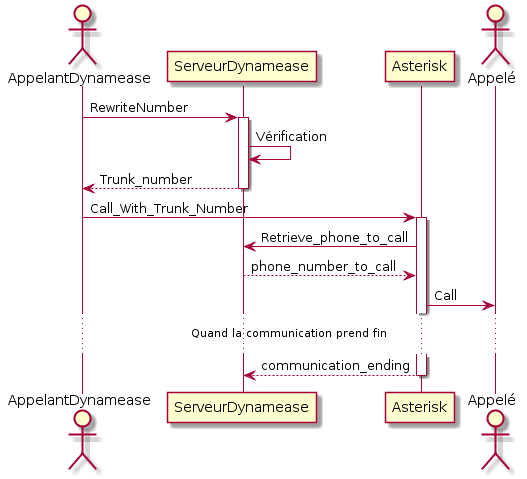
\includegraphics[scale=0.8]{img/sequence_rewirte.png}
	\caption{\label{sequence_rewirte} Diagramme de séquence de la réécriture de numéro}
\end{figure}

Nous voyons sur ce diagramme que le procédé est initié par les applications téléphoniques, nous allons donc commencer par la présentation du fonctionnement des requêtes utilisées par les applications téléphoniques.
\newpage

\begin{figure}[!h]
	\centering
	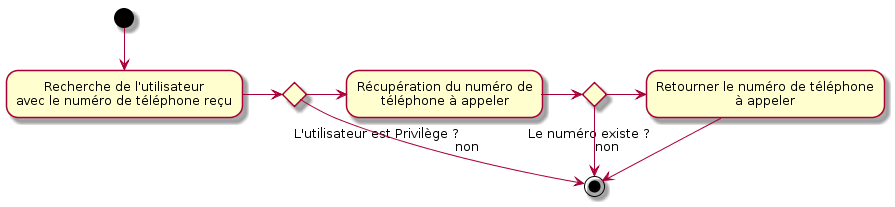
\includegraphics[scale=0.5]{img/activity_rewrite_ast.png}
	\caption{\label{activity_rewrite_ast} Diagramme d'activité de la méthode appelée par le serveur Asterisk}
\end{figure}


L'application téléphonique devra envoyer une requête au serveur pour indiquer que l'utilisateur souhaite effectuer une réécriture de numéro. Cette requête devra contenir le numéro à appeler ainsi que l'Id de l'utilisateur voulant passer l'appel. Une réponse est alors renvoyée avec le numéro de téléphone à joindre. L'application téléphonique aura alors pour rôle de lancer un appel vers ce numéro de téléphone.

Plusieurs choix sont possibles en ce qui concerne la réponse renvoyée lorsque la requête est envoyé de la part d'un utilisateur non privilège. Soit nous renvoyons une requête indiquant à l'utilisateur qu'il ne détient pas des droits nécessaires pour effectuer ce genre d'appel. Soit nous renvoyons les numéros de téléphone passés en paramètre de la requête. C'est cette dernière qui est choisie, car elle permet quand même à l'appel d'être effectué.

Le numéro à appeler sera stocké en mémoire du serveur dans un objet de type dictionnaire, ayant pour clef l'identifiant du client privilège et pour valeur le numéro à appeler. Ainsi nous permettons aux utilisateurs de pouvoir passer par l'historique d'appel de leur téléphone pour contacter le dernier contact appelé depuis leur numéro Dynamease.\\

On a noté dans la partie précédente les différentes informations que devait détenir le serveur téléphonique. Les différents numéros d'un utilisateur Dynamease sont stockés sur le serveur. Il est donc aisé de récupérer ces informations, afin de déterminer si un numéro entrant appartient à l'utilisateur. De plus les numéros de Trunk peuvent être considérés comme des constantes. Il est donc préférable que celles-ci soient stockées dans les fichiers de configuration du serveur Dynamease. En revanche cette technique ne marchera que pour le dernier contact appelé grâce à la réécriture de numéro. Pour rappeler des anciens contacts il faudra, soit passer par l'historique d'appel de Dynamease, la liste de contact ou l'option numérotation de Dynamease.
\newpage
\begin{figure}[!h]
	\centering
	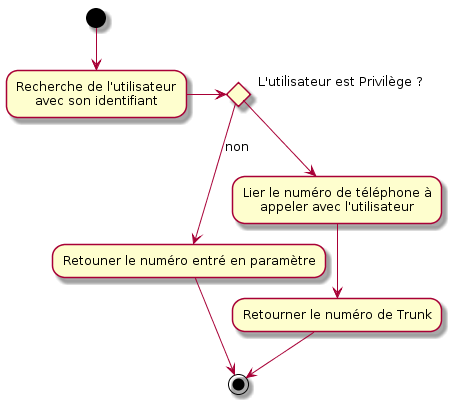
\includegraphics[scale=0.7]{img/activity_rewrite_app.png}
	\caption{\label{activity_rewrite_app} Diagramme d'activité de la méthode appelée par les applications téléphoniques}
\end{figure}

La meilleure solution est de créer une requête permettant au serveur téléphonique de vérifier si un numéro correspond à un utilisateur donné et s'il détient les droits privilèges. La réponse renvoyée correspondra au numéro que l'utilisateur Privilège souhaite joindre. Si l'appel ne provient pas d'un utilisateur Privilège, la réponse indiquera au serveur téléphonique de mettre fin à l'appel. Cette requête sera effectuée à chaque appel entrant sur le Trunk présent sur le serveur téléphonique.

\subsubsection{Les applications téléphoniques}

Les applications téléphoniques doivent envoyer une requête vers le serveur Dynamease dès que l'utilisateur sélectionne l'appel d'un contact. L'application doit également fournir le numéro à appeler.

Avant tout envoie de requête, une vérification sur le type de contact de l'utilisateur est effectuée. Que ce soit pour Iphone ou pour Android, le stockage des informations de l'utilisateur est géré de la même manière. Un procédé de type clef valeur (dictionnaire) persistant est présent sur les deux applications. Ce dictionnaire est rempli lors de la connexion de l'utilisateur. Il nous suffit donc ici de vérifier si l'utilisateur détient bien les droits avant d'envoyer cette requête. Bien que le serveur effectue également cette vérification, il est important d'effectuer cette vérification en amont pour ne pas surcharger le serveur de requêtes inutiles.\\

Dans les deux applications, les contacts sont rangés en deux catégories, les contacts Dynamease et les contacts du téléphone. Les contacts du téléphone sont pourvus d'un numéro de téléphone alors que les contacts Dynamease n'ont que leur identifiant Dynamease. Donc selon le contact à appeler, l'application doit soit envoyer un numéro de téléphone ou le numéro de l'identifiant Dynamease du contact.

\section{Le Click2Call}

Le Click2Call sera proposé comme une option, limitée dans le temps, pour tous les clients Dynamease. Cette option permettra aux clients de disposer de cartes de visite virtuelles publiques, qu'ils pourront déposer sur des sites internet. Ces cartes de visite permettront aux clients d'être contactés grâce à elle en un seul clique. Cet appel se fera sans échange de numéro de téléphone. C'est-à-dire que l'appelant ne verra pas le numéro du client et inversement.

\subsubsection{Étude du cahier des charges}

Pour réaliser cette fonctionnalité nous avons besoin de mettre en relation deux personnes sans échange de numéro. Le serveur téléphonique sera utilisé afin de créer un lien entre les deux communicants. Je ne serais, encore une fois, pas en charge de cette partie du développement mais nous aborderons le fonctionnement global de cette partie.

Nous allons avoir besoin du serveur Dynamease qui sera en charge d'orchestrer les échanges d'informations avec le serveur téléphonique et les applications téléphoniques.

Les applications téléphoniques devront également être changées dans le but de pouvoir recevoir les informations des appels.

\subsubsection{Fonctionnement du serveur téléphonique}

Le serveur téléphonique aura pour charge, la liaison entre les deux interlocuteurs grâce à des conférences. Ces conférences ne seront accessibles que par l'appelant et l'appelé, une requête est donc créée pour récupérer les conférences liées aux numéros de téléphone renseignés. Les conférences sont désignées par un identifiant unique, leur nom.

Pour accéder à une conférence, il faut faire intervenir un numéro de Trunk. C'est ce numéro qui sera affiché sur les appareils téléphoniques des deux interlocuteurs, car leur appel se fera vers le numéro de Trunk. Ainsi aucun des deux interlocuteurs n'aura le numéro de téléphone de l'autre interlocuteur.

\subsubsection{Le serveur Dynamease}

Le serveur Dynamease aura pour rôle la gestion du fonctionnement du Click2Call. Nous avons vu précédemment qu'il faut créer des conférences pour chacun des appels. Ces conférences devront donc être créées et stockées jusqu'à leur destruction. Un cycle de vie nous servira donc pour gérer toutes ces conférences et éviter une surcharge du serveur.

Les conférences passent par plusieurs étapes. La première étape est la création, à ce moment la conférence est ajoutée à la liste des conférences et est identifiée par un nom unique (ce nom est généré aléatoirement). Par la suite, la conférence passe en attente, c'est-à-dire que cette conférence est à disposition pour être utilisée par le serveur téléphonique. Lors de l'utilisation de cette conférence, son statut passe en mode attribué, dans ce cas-là elle ne peut plus être attribuée, jusqu'à ce que cette conférence soit terminée. Une fois terminée, la conférence repasse en attente. Ainsi on peut réutiliser plusieurs fois la même conférence est ainsi réduire le nombre d'objets conférence à stocker en mémoire.

Avant l'attribution de conférence on vérifie que le client Dynamease appelé n'est pas déjà présent dans une autre conférence. Ainsi on peut avoir une meilleure gestion des conférences, et identifier la disponibilité de l'utilisateur.

La liste de conférence, peut être accédée à tout moment, il faut donc gérer les problèmes de concurrence sur cette liste. On utilise donc la synchronisation des méthodes fournie par Java. Ces méthodes permettent de gérer l'accès à une liste par plusieurs Threads. Cette méthode gère une liste FIFO (First In First Out) de Thread, la liste n'est accessible que par un seul Thread à la fois, ce qui permet d'éviter les problèmes de concurrence.\\

L'accès à la conférence peut se faire de deux manières, soit par un appel vers le numéro du Trunk, soit un appel est émis de la conférence vers un utilisateur. La personne appelante utilisant le Click2Call sera forcément amenée vers la conférence, par un appel vers celle-ci. En ce qui concerne l'utilisateur Dynamease, il faut décider de la manière dont il sera amené vers la conférence.

En passant l'appel depuis la conférence, l'application Dynamease n'aura qu'à afficher les informations clients, comme elle le fait habituellement. En utilisant la seconde solution, l'application Dynamease devra effectuer un appel vers la conférence, mais les charges d'appel pour Dynamease seront diminuées. Pour des raisons économiques, c'est ce second choix qui sera utilisé. De plus avec cette seconde solution, le prix de cette option pourra s'effectuer grâce à des appels surtaxés.\\

La procédure utilisée par cette fonction est la suivante :

\begin{figure}[!h]
	\centering
	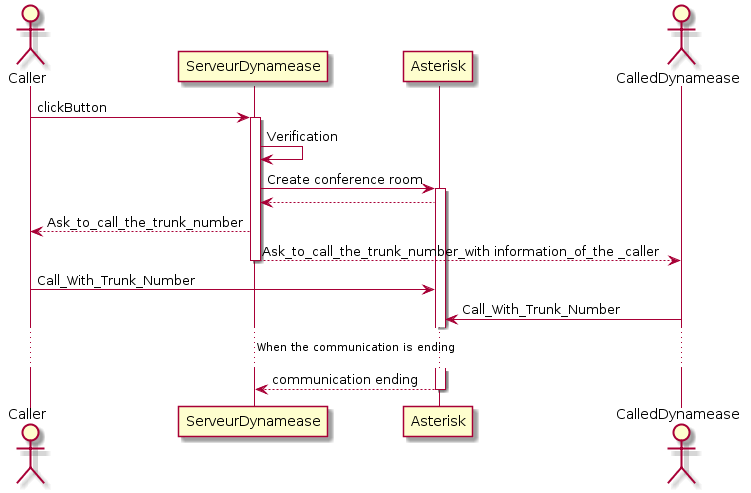
\includegraphics[scale=0.7]{img/sequence_click2call.png}
	\caption{\label{sequence_click2call} Diagramme de séquence de la fonctionnalité du Click2Call}
\end{figure}

Une personne appuie sur le bouton Click2Call. Ce bouton envoie une requête au serveur Dynamease contenant l'identifiant de l'utilisateur Dynamease à appeler ainsi que le contexte dans lequel s'effectue l'appel (type de site, objet vendu ...). À la réception de la requête, le serveur Dynamease vérifie qu'il existe des conférences disponibles, s'il n'en existe pas le serveur en crée une nouvelle et demande sa création au serveur téléphonique. Ensuite le serveur vérifie si l'utilisateur à joindre est disponible. Si cette vérification s'est effectuée sans problème, l'objet conférence est modifié avec les informations sur les numéros de téléphone pouvant y accéder. Le numéro du Trunk est envoyé à l'appelant. Ensuite une notification du type Click2Call est envoyée à l'utilisateur Dynamease avec le numéro de la conférence et les informations de cet appel.

La conférence démarre dès que les deux protagonistes entrent dans la conférence. Elle se termine quand un des deux protagonistes coupe la communication. À la fin de cette conférence une requête est envoyée au serveur Dynamease pour l'informer que la conférence peut être réattribuée.\\

En plus de ces requêtes, d'autres requêtes, spécifique à Dynamease, ont été créées dans l'objectif de gérer les différents numéros de conférence. Ajouter des numéros de conférence, et lister les informations pouvant être récupérées sur les numéros de conférence.

\subsubsection{Les applications téléphoniques} 

Les applications téléphoniques doivent, à l'arrivée d'une notification Click2Call, générer un appel vers le numéro de Trunk, dans le but d'accéder à la conférence.

Dans cette notification il doit être présent les informations sur l'appelant. Pour cela on utilise le même principe déjà existant sur les notifications d'appel.\\

La gestion des notifications étant différentes selon le système d'exploitation il est important de bien différencier les deux types de notification. Nous allons commencer par les applications Android.

Les notifications d'appel, sont affichées par le biais du système Toast. Un toast est une fenêtre s'affichant obligatoirement au premier plan. La fenêtre Toast est donc affichée au premier plan même lors d'un appel, ce qui permet aux utilisateurs de lire les informations même si la fenêtre d'appel est affichée. Cette fenêtre est affichée pendant une courte durée, mais il est possible de laisser cette fenêtre affichée plus longtemps en utilisant le principe de \textit{timer} pour demander l'affichage du Toast à intervalles de temps réguliers. Les informations sont donc affichées pendant un laps de temps suffisamment long pour que l'utilisateur puisse lire toutes les informations récupérées sur l'appelant.

Lors de la réception de cette notification, l'utilisateur doit décider s'il veut répondre à l'appel. Ce qui signifie que la notification doit permettre la gestion d'actions de la part de l'utilisateur. Android ne permet pas la gestion des actions avec les Toasts. Cette notification doit simuler un appel. Un appel sur Android est représenté par une vue en plein écran. On peut reprendre ce principe en créant une activité. Cette activité affichera les informations de l'appelant, ainsi que deux boutons pour laisser le choix à l'utilisateur d'accepter ou de refuser l'appel.

Il est également possible de récupérer certaines informations de l'utilisateur comme la sonnerie utilisée par défaut des appels. On peut donc faire retentir cette sonnerie afin que l'utilisateur ait la sensation d'un appel. La fenêtre suivante est affichée sur le portable

\begin{figure}[!h]
	\centering
	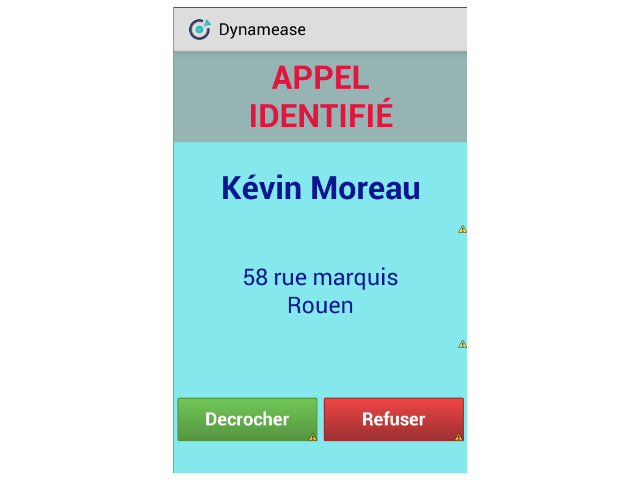
\includegraphics[scale=0.7]{img/click2call.png}
	\caption{\label{notification_click2call}Notification Click2Call}
\end{figure}


En appuyant sur le bouton répondre, la fenêtre se ferme, et un appel est émis vers le numéro de conférence. Ainsi l'expérience utilisateur n'est pas altérée, car la sensation d'appel reste la même.\\

En ce qui concerne l'application Iphone, il est impossible d'avoir la même expérience utilisateur que pour la partie Android. Il n'est pas possible d'afficher des notifications spéciales si l'application n'est pas au premier plan. La notification Click2Call doit donc être affichée comme une notification Iphone normale. Comme pour l'application Android, il faut laisser le choix à l'utilisateur de répondre ou non à l'appel. Pour cela une fonctionnalité récente de IOS, disponible depuis la version 8, permet d'ajouter des boutons d'actions aux notifications. En ce qui concerne la notification sonore, il est possible d'avoir le même principe que les applications Android.


\section{L'appel depuis l'historique}

\begin{figure}[!h]
	\centering
	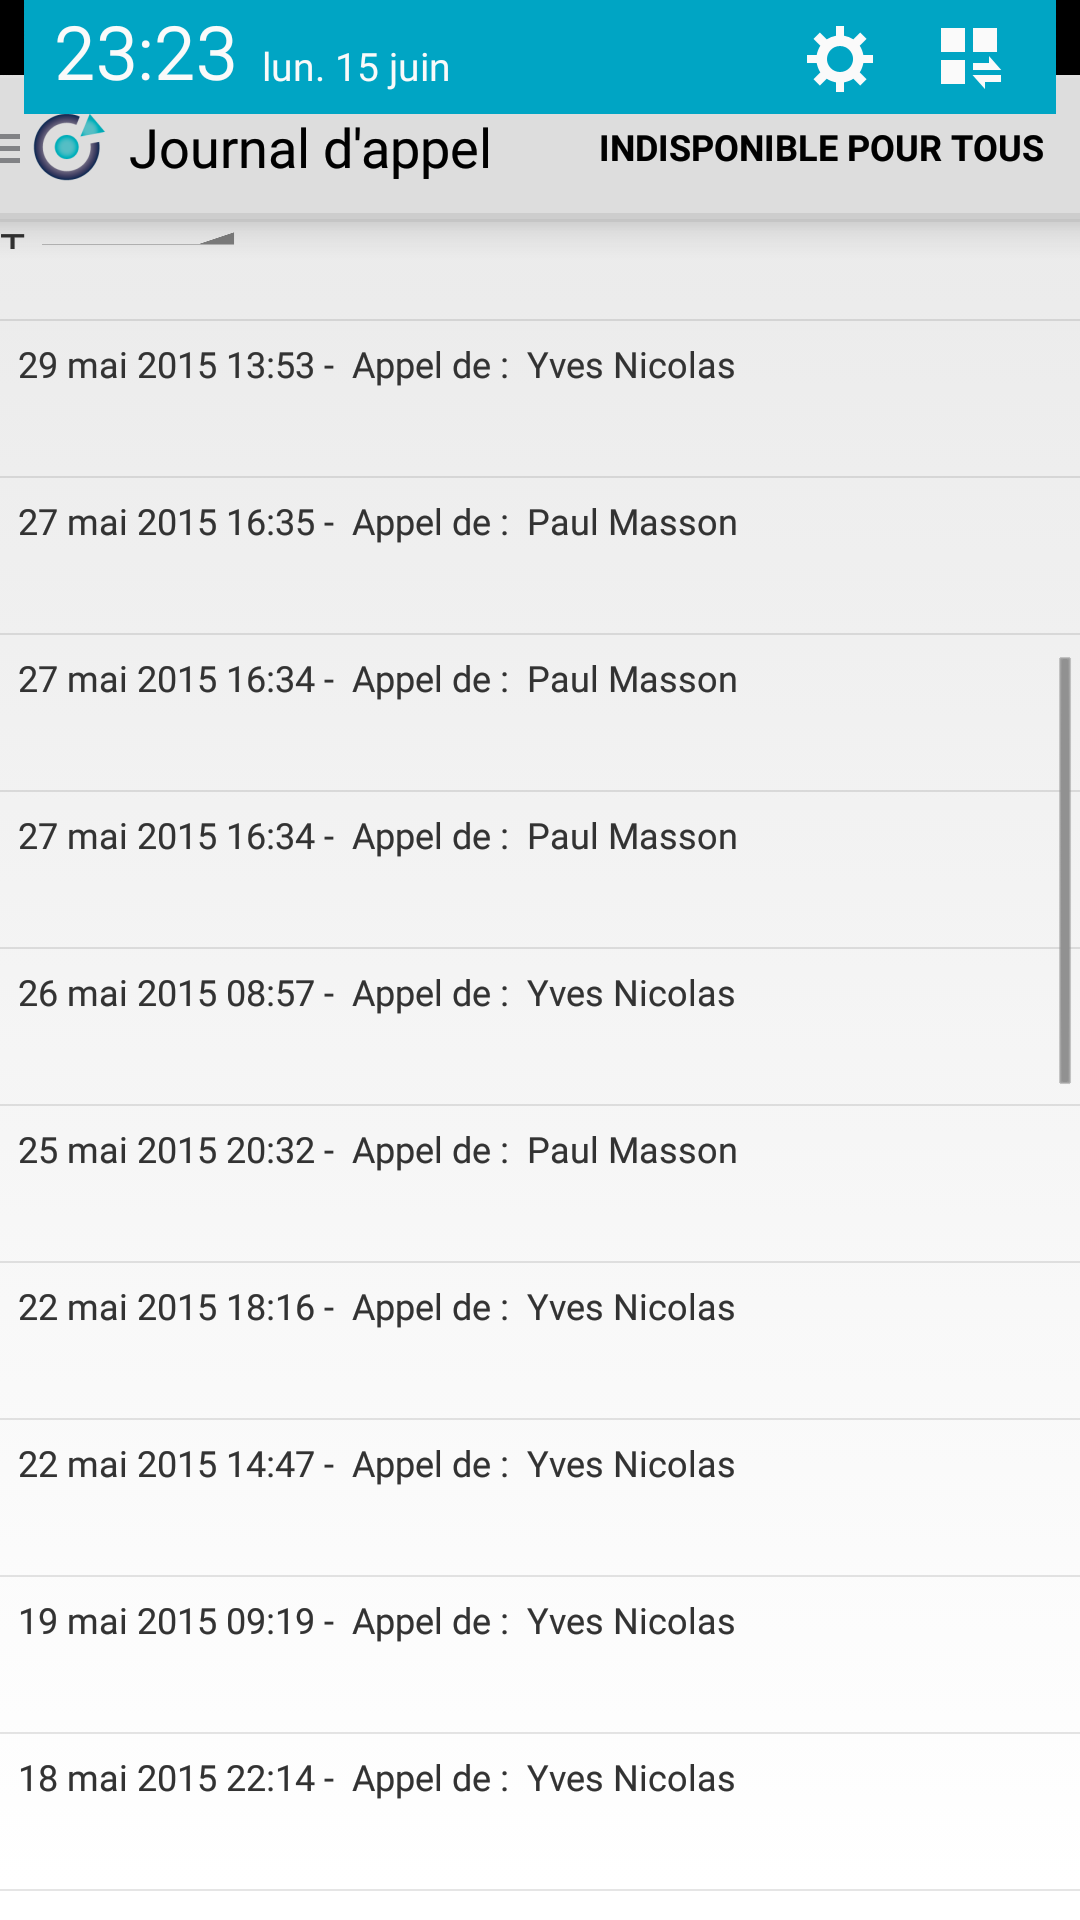
\includegraphics[scale=0.1]{img/historique.png}
	\caption{\label{historique} {Vue de l'historique d'appel sur l'application Android}}
\end{figure}

Les applications téléphoniques disposent d'un historique d'appel. Celui-ci nous indique la date et l'heure d'un appel, ainsi que d'éventuelles informations sur l'appelant. Par contre il n'est pas possible de rappeler les contacts depuis cet historique. Il est donc question de pouvoir effectuer ce rappel.

\subsubsection{Étude du cahier des charges}

Pour réaliser cette fonctionnalité nous avons besoin de faire une modification sur la base de données MySQL. En effet, la table représentant les appels ne stocke pas les informations nécessaires au rappel du contact, comme le numéro de téléphone ou l'identifiant Dynamease. Il faut donc rajouter ces informations dans la base de données. Cette modification sera effectuée par une autre personne. Quant à moi je serais en charge des modifications à effectuer sur les applications téléphoniques.

Je dois faire les modifications nécessaires pour que les applications téléphoniques gèrent cette nouvelle fonctionnalité.

\subsubsection{Les modifications}

La récupération des informations nécessaires se fait via un objet Json. Le traitement de cet objet est différent selon le système d'exploitation téléphonique.

Pour les applications Android, le traitement se fait via un Mapper. Le Mapper est chargé de traduire une chaîne de caractères formée comme un objet Json en un autre objet passé en paramètre. L'objet Json, pour rappel se présente comme un dictionnaire (clefs, valeurs). Les clefs représentent les noms de variable et les valeurs, les valeurs prises par les variables.

En ce qui concerne les applications Iphone, le procédé est manuel. L'objet voulu doit être récréé, contrairement à Android, où l'objet utilisé est le même que celui utilisé sur le serveur Dynamease.

Maintenant que ces informations sont récupérées, il suffit simplement d'effectuer les mêmes tâches que pour un appel depuis la liste de contact.

\subsubsection{Amélioration de la base de données}

Après cette mise en place j'ai observé les modifications de la base de données. J'ai remarqué quelques erreurs effectuées sur celle-ci.

\newpage
\begin{figure}[!h]
	\centering
	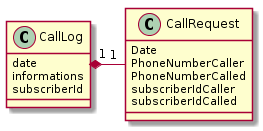
\includegraphics[scale=1]{img/classeCallLogOld.png}
	\caption{\label{class_callLog_old} Diagramme de classes de la table représentant l'historique d'appel}
\end{figure}

On voit que cette base de données ne respecte pas le terme de clef unique en effet. Il est possible que la valeur de date soit identique pour deux entrées.

La cardinalité entre ces deux tables, signifie que les informations présentent sur $"call_request"$ pourraient être présente sur la table $"call_log"$

Je pense donc que la partie de la base de données représentant l'historique d'appel pourrai être remplacé par la table suivante :

\begin{figure}[!h]
	\centering
	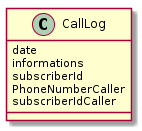
\includegraphics[scale=1]{img/classeCallLogNew.png}
	\caption{\label{class_callLog_new} Proposition d'amélioration du diagramme de classes de la table représentant l'historique d'appel}
\end{figure}

La première solution fût prise pour éviter les modifications sur une table déjà existante et risquer de perdre des données clients. 

 \chapter{La sécurité}
	Pour cette partie de travail, je n'avais pas de cahier des charges à proprement parler. J'étais beaucoup plus libre dans mes choix. Il fallait que je m'organise dans le but de faire une gestion pour la sécurité de Dynamease. 

Le résultat à obtenir était de lister les éventuels failles de sécurité et de proposer des moyens pour les résoudre. Dans le but de déceler ces éventuels failles j'ai suivi les étapes suivantes :

\begin{enumerate}
	\item Observation du code de sources de l'application;
	\item Lister les éventuels failles critiques qui pouvaient être présentes;
	\item Effectuer les manipulations a fin de trouver la faille;
	\item Détecter la source de cette faille;
	\item Déterminer les solutions à ce problème.
\end{enumerate} 

En plus de trouver et résoudre ces différentes failles, je me devais également de penser à mettre en place le protocole Https pour le site web de Dynamease. Cette mise en place devra être effectué par une jeune décrocheur, je serais par contre en charge de jouer le rôle de chef de projet, en lui indiquant ce qu'il doit faire, et également jouer le rôle de formateur, en lui apprenant les différentes méthodes pour arriver à l'objectif. 

\section{Vérification de sécurité des services Dynamease}

Dans cette partie j'expliquerais, pour toutes les failles de sécurité que j'ai pu trouver, les méthodes utilisées pour trouver celles-ci.

\subsection{Requêtes non sécurisées}

\subsection{Cookies non sécurisés}

Lors de l'utilisation de l'outil de mise en place d'un environnement Dynamease, je me suis aperçu qu'en changeant les données de la base de donnée une connexion utilisateur était établie, alors que l'utilisateur connecté n'existait pas sur la base de donnée précédente.

La question qui se posait alors, était qu'est ce qui déterminait qu'un utilisateur est connecté. Le serveur Dynamease détermine la connexion grâce aux cookies.

Après une observation des cookies, il est apparu que les informations contenues dans les cookies était écris en claires. L'information qui nous intéresse est l'Id Dynamease. L'identifiant Dynamease étant unique c'est grâce à celui-ci que l'utilisateur peut être identifié.

Cette information étant en claire il suffit donc de la modifier avec un autre identifiant afin d'usurper le compte d'un autre utilisateur.
\\\\

Afin de régler cette faille il suffit d'encoder les informations contenues dans les cookies. De plus d'autres informations devraient être contenue dans les cookies afin d'être certain que l'Id utilisé représente bien l'utilisateur actuel. 

\subsection{Sauvegarde des données}

\section{Mise en place d'un certificat Https}

Les communication vers le site web de Dynamease s'effectuait par le biais du protocole http. Ce protocole n'est pas sécurisé, pour protéger les données des clients Dynamease. Il a été décidé de mettre en place le protocole https, qui chiffre les communications avec les clients.

Le protocole https, fonctionne sur le principe clef publique clef privée. Une clef publique est envoyé à chacun des clients pour chiffrer les données que celui-ci envoi. Ces données ne peuvent être alors décrypté uniquement par la clef privée qui reste sur le serveur.

Cette mise en place sera réalisé par un jeune décrocheur que je devrais superviser. J'aurais pour charge de lui indiquer ce qu'il devra faire, et le mettre sur la voie pour qu'il devienne autonome dans son travail.

\subsubsection{Étude du cahier des charges}

Ce protocole doit être mis en place sur les serveur existants. La communication entre les utilisateurs et le serveur Tomcat est orchestré par Nginx.

Nginx est un reverse proxy. Celui-ci permet de redirigé les requêtes des utilisateurs vers les plateformes appropriées. Il est également possible grâce à Nginx de redirigé toutes les requêtes d'un serveur vers un autre serveur, ce qui est extrêmement utile pour des migrations.

Il faudra donc que ce soit Nginx qui gère la gestions des différentes clefs du protocole https. La configuration de Nginx sera donc essentielle dans la suite de cette mise en place.\\

Les clefs doivent également être certifiées. Les noms de domaines nous sont fournie par le bureau d'enregistrement de nom de domaines Gandi. Cette société fournie également des certificats de sécurité. Il faudra donc également faire la procédure d'obtention d'un de ces certificats.

\subsubsection{Mise en place de la formation}

Pour réaliser cette mise en place j'ai décidé de faire passer ce jeune décrocheur par trois étapes :

\begin{enumerate}
	\item Mise en place d'une configuration standard Nginx;
	\item Mise en place d'une clef non certifiée;
	\item Mise en place d'une clef certifiée Gandi.
\end{enumerate}

Pour la première étape, je lui fournirais toutes les documentations officielles nécessaires à la réalisation de cette première étape. Et au fur et à mesure de la formation je diminuerais le nombre de documentations fournies pour l'obliger à aller rechercher l'information utile.

Les test qui seront effectués par le décrocheur se dérouleront sur un serveur à part afin de pouvoir assurer un fonctionnement normal du reste des infrastructures en cas d'erreur.\\\\

Nous aborder en détail la mise en place du certificat. Pour ce faire nous avions plusieurs choix au niveau du type des certificats. Nous pouvions soit choisir un certificat pour un seul nom de domaine, qui incluait le sous-domaine $"www"$. Ou alors choisir, le certificat wildcard, qui permet de certifier un domaine et tout les sous-domaine. C'est ce type de produit que nous avons choisi dans le but de pouvoir l'intégrer dans tout nos serveurs, ainsi que ceux de tests, ce qui rendrait les tests de pré-production plus réaliste.

Pour demander un certificat il faut d'abord créer une clef. Cette clef une fois créée avec les informations nécessaire sera ensuite passé à Gandi qui nous fournira le certificat associé à cette clef. Une fois ce certificat créé il nous suffit de configurer Nginx afin qu'il utilise ce certificat.


 \chapter{Conclusion}
	Ayant déjà effectué mon stage technicien au sein de Dynamease, je n'ai eu aucun mal à m'intégrer dans l'entreprise. Ce qui eut pour effet de pouvoir commencer au plus vite le travail qui m'était confié. De plus le fait de connaître en amont les différents employés de Dynamease m'a permis d'être beaucoup plus social avec eux et n'avoir aucun mal à mettre en avant mes idées, ou de poser diverses questions.\\

Le fait de développer une application sur deux systèmes d'exploitation différents fut très intéressant. Avoir deux points de vu différents d'une même réalisation, m'a obligé à mettre plus d'importance sur la conception et sur la recherche de technologies sur les deux systèmes. De plus le développement sur IOS est limité par Apple, pour des raisons de qualité des applications. Cette limite m'a obligé à être le plus inventif possible pour pouvoir la contourner et pouvoir réaliser une application plus ou moins identique à l'application Android. De plus la mise en production décalée entre les deux applications, du fait des vérifications effectuées par Apple, m'a également permis d'améliorer la gestion de mon temps de travail sur les deux applications, afin de pouvoir soumettre les deux applications aux utilisateurs en même temps.

Les différentes fonctionnalités à réaliser sont actuellement proposées aux clients Dynamease. Bien qu'en ce qui concerne la fonctionnalité du Click2Call, elle ne soit encore qu'au stade de prototype. L'objectif est rempli car il consistait à prouver qu'il était possible de fournir une telle fonctionnalité aux clients Dynamease. D'autres fonctionnalités ont été réalisé en parallèle de celles présentée, comme l'ajout de la numérotation Dynamease.\\

Le développement d'un outil permettant l'installation de l'environnement complet de Dynamease fut très intéressant de part du fait qu'il a fallu me former sur les différents éléments utilisés par Dynamease. Cet apprentissage m'a permis de comprendre toutes les technologies utilisées ainsi que leur utilité. D'une autre part le fait de réaliser des scripts intelligents permettant de réaliser une suite de commandes m'a toujours intéressé dans le sens où il faut réfléchir aux différents cas d'utilisation du script. Cet outil est complet et ne nécessite pas forcément d'améliorations, car il est actuellement utilisé par tous les employées de Dynamease ainsi que les consultants. Cependant un manuel d'utilisation pourrait être créé afin de faciliter encore plus l'utilisation de l'outil.\\

L'amélioration de la sécurité Dynamease m'a fait comprendre les enjeux de la cryptologie au sein d'une entreprise. La recherche de failles est un procédé très intéressant dans le sens où il faut observer toutes les parties de l'application en se forçant à avoir un œil extérieur et critique. C'est d’ailleurs durant la recherche de ces failles que j'ai pu remarquer quelques anomalies dans ce qui était réalisé, et sur les côtés non ergonomiques de certaines parties de l'application. De plus devoir apporter une solution et mesurer l'état critique de la faille, permet de se rendre compte des erreurs à éviter dans le développement d'une application. Me rendre compte de certaines erreurs sur ce service m'a permis de critiquer la fiabilité de chacune des fonctionnalités que je crée. Durant le reste de mon stage je devrais mettre en place les procédures pour régler ces différentes failles.\\

Les avantages du travail en startup sont que mon travail n'était pas bridé, je pouvais réaliser mes objectifs sans avoir de réelles contraintes. Les seules contraintes que je suivais étaient celles que je m'obligeais à suivre. Mon avis importait beaucoup dans la réalisation des fonctionnalités, je ne me sentais pas comme un stagiaire mais comme un employé à part entière dans l'entreprise Dynamease. Mon seul regret est de ne pas avoir été en contact avec plus d'employés développeur avec lesquels j'aurais pu discuter sur les différentes méthodes de travail à employer. Malgré ce point, je pense que le manque de ce partage m'a permis de former ma propre méthode de travail en réalisant mes propres erreurs. Ainsi je comprends l'enjeu de ma méthode et pourquoi elle est nécessaire.\\

Pour la suite de mon stage je devrais mettre en place les différents outils de mesure de performance afin qu'ils soient utilisables par Dynamease. De plus la réalisation du transfert d'appel n'a pas pu être effectuée par faute de temps, aussi bien sur les applications téléphoniques que sur les serveurs Dynamease et Asterisk.

Il est cependant difficile de déterminer les améliorations possibles des fonctionnalités ajoutées sachant que celles-ci ont plutôt été rapides à réaliser. Ces fonctionnalités ont donc eu le temps d'être corrigées et améliorée tout au long de ce stage.\\

La résolution des failles de sécurité, bien qu’intéressante n'a pas été réalisée durant cette première partie du stage. Leur priorité de réalisation était nettement moins importante que la réalisation des nouvelles fonctionnalités promises pour la version 3.0 de Dynamease. Cette version étant mise en place, j'aurais beaucoup plus de temps pour régler ces failles avant la fin de mon stage. J'aurais dû cependant mettre plus en avant l'importance de ces failles afin de les régler au plus vite, même si cela engendrait un retard sur la sortie de la version 3.0 de Dynamease. 

 \pageQuatriemeCouverture{}	
\end{document}
